%!TEX root = main.tex

\section{Experiments and numerical results}

\subsection{Experimental setup}
\begin{figure}[h!]
  \centering
    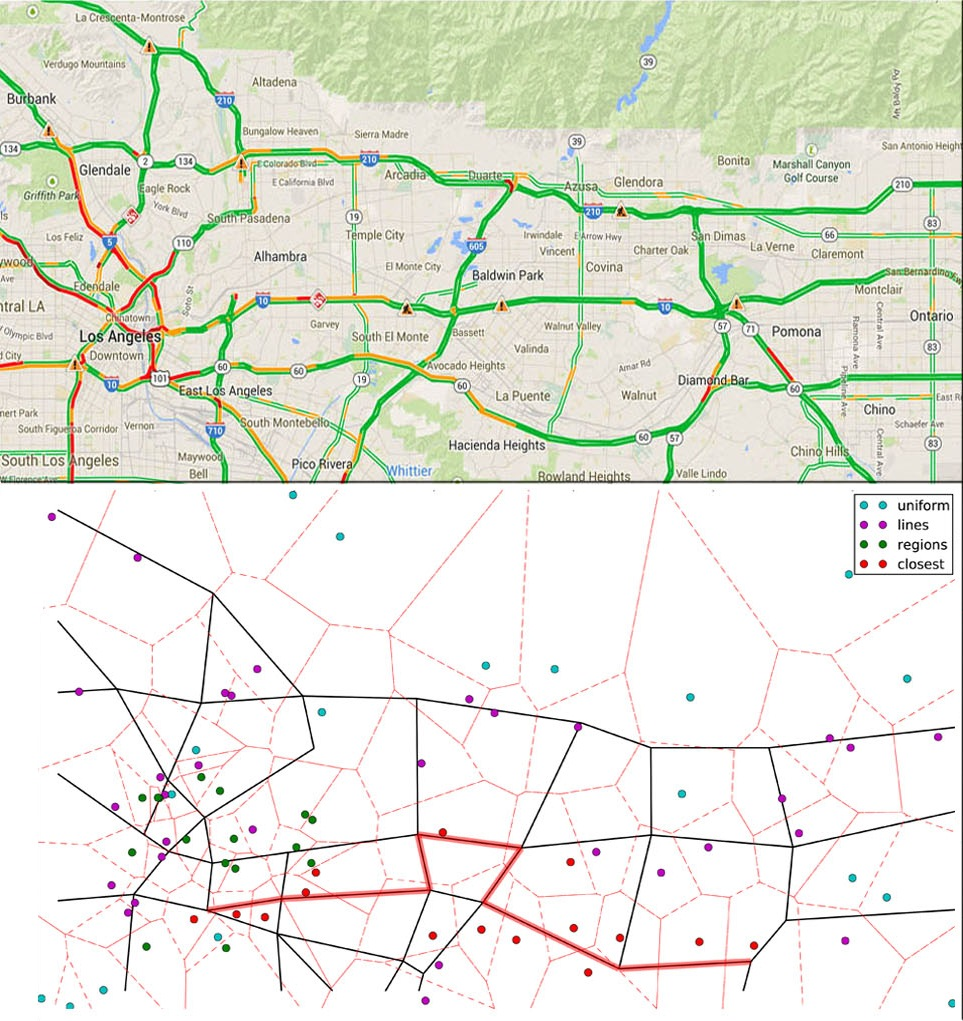
\includegraphics[width=0.47\textwidth]{figures/small_map_half.jpeg}
  \caption{\footnotesize{Benchmark example network based off of the Highway network of the I-210 highway corridor in L.A. county (top, from Google Maps); Network with 80 sampled cells, with a higher concentration of cells near downtown (bottom). A random path from is shown in red with the closest cell towers.}}
  \label{fig:small-network}
\end{figure}

We consider a medium sized network and the following scenarios
\begin{itemize}
\item \textbf{???} ($N=375$):
\item \textbf{City Center} ($N=375$): We emulate a popular commercial district with a dense sampling of cellular towers.
\end{itemize}

\subsection{Results}

“sparser”: smallest number of cell towers for which route flow accuracy is pretty good ($<5\%$ error); hopefully somewhat robust to handoff model

“city center”: super dense number of cell towers; handoff model should cause tons of problems here quickly

